\documentclass[russian, utf8]{eskdtext}
\newcommand*{\No}{\textnumero}
\ESKDdepartment{Кафедра Систем Управления и Информатики}
\ESKDcompany{Университет ИТМО}
\ESKDdocName{Устройство для измерения плотности жидкости}
\ESKDsignature{КСУИ.150.P3340.001 ПЗ}
\ESKDauthor{Овчаров А.О.}
\ESKDchecker{Бойков В.И.}
\ESKDnormContr{Бойков В.И.}
\ESKDcolumnIX{\small Университет ИТМО\\
Кафедра СУиИ}

\usepackage[hidelinks]{hyperref}
\usepackage{pscyr}

\usepackage{tocloft}
\renewcommand{\cftaftertoctitle}{\hfill}
\renewcommand{\cfttoctitlefont}{\hspace{7cm}\Large\bfseries}	%KOSTIL'
\renewcommand{\cftaftertoctitle}{\hfill}
\renewcommand{\cftdot}{.}
\renewcommand{\cftsecleader}{\cftdotfill{\cftdotsep}} % for sections

\usepackage{wrapfig}
\usepackage{graphicx}
\graphicspath{{images/}}
\DeclareGraphicsExtensions{.pdf, .jpg, .png}

\usepackage{caption}
\captionsetup[table]{singlelinecheck=false}		% Заголовок таблиц слева
\captionsetup[table]{aboveskip=2pt,belowskip=2pt}			%belowskip=6pt 	% Позиционирование заголовка

% Рисование 
\usepackage{tikz}

\begin{document}
\tableofcontents
\thispagestyle{empty}
\newpage

% Introduction ------------------------------------------------------------
{\section*{Введение}
\addcontentsline{toc}{section}{Введение}}

В данной курсовой работе, в соответствии с полученным заданием, требуется разработать модуль управления для бесколлекторного электропривода постоянного тока на базе микроконтроллера, отвечающим следующим требованиям: 
\begin{itemize}
	\item тип двигателя - 3х фазный бесколлекторный
	\item способ управления - коммутация обмоток
	\item обратная связь - датчики Холла
	\item режимы - Пуск, Останов., Выбор скорости
	\item микроконтроллер - ATMEL
	\item связь с компьютером - RS 232
	\item гальваническая развязка линии связи с компьютером
	\item питание - 12 вольт постоянного тока
\end{itemize} \par
У бесколлекторного двигателя постоянного тока (БДПТ), по сравнению с обычными двигателями постоянного тока достаточно много плюсов. Главным его достоинством является отсутствие щеточно-коллекторного узла, что сильно увеличивает надежность и время эксплуатации двигателя. Также из-за отсутствия щеточно-коллекторно узла увеличивается диапозон изменения скоростей, уменьшаются массо-габаритные показатели и увеличивается КПД, поскольку отсутствуют потери на щеточно-коллекторном узле. \par

Едиственным большим минусом, из-за которого еще не отказались от обычных двигателей постоянного тока, это достаточно большой по габаритам и сложный блок управления, регулятор. Без него нельзя запустить двигатель, поскольку для минимально работы требуется перключать фазы БДПТ в определенный момент времени.\par

Регулятор состоит из силового каскада, который коммутирует обмотки в определенный момент времени. Сам каскад управляется коммутирующим устройством, генерирующим последовательность импульсов (ЧИМ) определенной частоты. Для того, чтобы просто запустить двигатель этого достаточно. Но чаще всего необходимо регулировать скорость двигателя. Cамым простым, неточным и дешевым способом является использование датчиков Холла. Они позволяют качественней коммутировать обмотки, а также вычислять скорость двигателя. \par

Благодаря высокой надёжности и хорошей управляемости, бесколлекторные двигатели применяются в широком спектре приложений: от компьютерных вентиляторов и CD/DVD-приводов до роботов и космических ракет. Также этот тип двигателей часто используется в квадрокоптерах. Широкое применение БДПТ нашли в промышленности, особенно в системах регулирования скорости с большим диапазоном и высоким темпом пусков, остановок и реверса; авиационной технике, автомобильном машиностроении, биомедицинской аппаратуре, бытовой технике и проч. \par

\newpage
%% Functional scheme of BLDC motor ------------------------------------------
\section{Функциональная схема}
Функциональная работа системы изображена на рисунке 1.
\begin{figure} [h!]
	\centering
	\begin{tikzpicture}
		%\draw[gray, dotted] (0, 0) grid (15, 6);
		\draw[thick] (0, 2.5) -- (0, 3.5) -- (1, 3.5) -- (1, 2.5) -- (0, 2.5); \draw (0.5, 3) node {ЗУ};
		% Kontroller
		\draw[thick, ->] (1, 3) -- (2, 3) node[anchor = south east] {$\omega_d$};
		\draw[thick] (2, 2.5) -- (2, 3.5) -- (3.5, 3.5) -- (3.5, 2.5) -- (2, 2.5); \draw (2.75, 3) node {МКР};
		% Transistors
		\draw[thick, ->] (3.5, 3) -- (5, 3) node[anchor = south east] {$U_p$};
		\draw[thick] (5, 2.5) -- (5, 3.5) -- (6, 3.5) -- (6, 2.5) -- (5, 2.5); \draw (5.5, 3) node {СК};
		% Motor
		\draw[thick, ->] (6, 3) -- (7.5, 3) node[anchor = south east] {$U_\text{фаз}$};
		\draw[thick] (7.5, 2.5) -- (7.5, 3.5) -- (9.5, 3.5) -- (9.5, 2.5) -- (7.5, 2.5); \draw (8.5, 3) node {БДПТ};
		% Feedback
		\draw[thick, ->] (8.5, 2.5) -- (8.5, 1.5) -- (2.75, 1.5) -- (2.75, 2.5) node[anchor = north east] {$S$};
	\end{tikzpicture}
	\vspace{0.5cm}
	\caption{Функциональная схема}
\end{figure} \par

В режиме регулирования скорости вращения вала двигателя задающее устройство \textbf{ЗУ} генерирует последовательный восьмеричный код, который подается на микроконтроллер \textbf{МКР}. В микроконтроллере, на основании показаний с датчиков холла $S$ и желаемой скорости $\omega_d$, генерируются импульсы управления $U_p$, которые коммутируют транзисторы силового каскада \textbf{СК}, тот в свою очередь коммутирует бесколлекторный двигатель постоянного тока \textbf{БДПТ}. На БДПТ находятся датчики Холла, которые реагируют на магнитное поле ротора и посылают ипульсы $S$ на микроконтроллер. \par

Давайте подробней рассмотрим работу каждой из частей.

\subsection{Задающее устройство}

Задающее устройство состоит из АЦП и простой схемы регулировки напряжения, которая состоит из конденастора и потенциометров. \par
На устройство регулировки подается напряжение, которое зависит от диапозона работы АЦП. Регулируя ручку потенциометра мы благодаря конедсатору плавно меняем напряжение на выходе устройства регулирования. Полученное напряжение поступает на восьмибитный АЦП, после чего полученный параллельный код поступает на микроконтроллер. Данное напряжение пропорционально желаемой угловой скрорости двигателя.

\subsection{Микроконтроллер}

Самой важной частью всей схемы ялвяется микроконтроллер. Он следит за точностью коммутации обмоток двигателя и выполнения заданной угловой скорости. Данные действия происходят по схеме, изображенной на рисунке 2.
\begin{figure} [h!]
	\centering
	\begin{tikzpicture}
		%\draw[gray, dotted] (0, 0) grid (15, 6);
		\draw[thick, ->] (1, 3) -- (2.75, 3) node[anchor = south east] {$\omega_d$};
		\draw[thick] (3, 3) circle (0.25); 
		\draw[thick] (2.82, 2.82) -- (3.18, 3.18); \draw[thick] (3.18, 2.82) -- (2.82, 3.18);
		\draw[fill] (3, 3) -- (3.18, 2.82) arc(315:225:0.25) -- (3, 3);
		\draw[thick, ->] (3.25, 3) -- (4.5, 3) node[anchor = south east] {$e$}; 
		\draw[thick] (4.5, 2.5) -- (4.5, 3.5) -- (6, 3.5) -- (6, 2.5) -- (4.5, 2.5); \draw (5.25, 3) node {РГ};
		\draw[thick, ->] (6, 3) -- (7, 3);
		\draw[thick] (7, 2.5) -- (7, 3.5) -- (8.5, 3.5) -- (8.5, 2.5) -- (7, 2.5); \draw (7.75, 3) node {ГН}; 
		\draw[thick, ->] (8.5, 3) -- (10, 3) node[anchor = south east] {$U_p$};
		\draw[thick, ->] (9, 1) -- (3.75, 1);
		\draw[thick, ->] (7.75, 1) -- (7.75, 2.5);
		\draw[fill] (7.75, 1) circle (0.07cm) node[anchor = south west] {$S$};
		\draw[thick] (2.25, 0.5) -- (2.25, 1.5) -- (3.75, 1.5) -- (3.75, 0.5) -- (2.25, 0.5); \draw (3, 1) node {КС};
		\draw[thick, ->] (3, 1.5) -- (3, 2.75) node[anchor = north west] {$\omega_a$};
	\end{tikzpicture}
	\caption{Функциональная схема работы микроконтроллера}
\end{figure}

С АЦП приходит сигнал на порт микроконтроллера. Данный сигнал пропорционален желаемой угловой скорости $\omega_d$. Эта скрость сравнивается с реальной скростью двигаетля $\omega_a$ и получившаяся ошибка подается на регулятор РГ, который в соответствии с законом управления выбирает частоту, с кторой уже генератор ГН выполнит коммутацию транзисторов СК. \par

С датчиков холла БДПТ поступает сигнал $S = [S_1, S_2, S_3]$. На их основе выполняется коммутация транзисторов силового каскада, управляющего двигателем. Также зная расположение датчиков Холла в двигателе можем определить реальную угловую скрость $\omega_a$.

\subsection{Силовой каскад}

Силовой каскад трехфазного БДПТ представляет собой каскад из трех частей, каждая из которых состоит из двух последовательно соединенных транзисторов, между которыми подключается фазный провод БДПТ. Сами части параллельно подключаются к питанию. Схема такого каскада изображена ниже на рисунке 3.

\newpage

\begin{figure} [h!]
	\centering
	\includegraphics[angle = -90, width = 0.9\textwidth]{BITransistors.pdf}
	\caption{Схема силового каскада трехфазного БДПТ}
\end{figure}

Коммутация происходит от обмотки к обмотки, тоесть положительний потенциал подается последовательно к A-B-C обмоткам. При этом отрицательный потенциал чередуется. В итоге получается слуедующий алгоритм коммутации: AB-AC-BC-BA-CA-CB-AB-... Графически это представлено ниже.

\begin{figure} [h!]
	\centering
	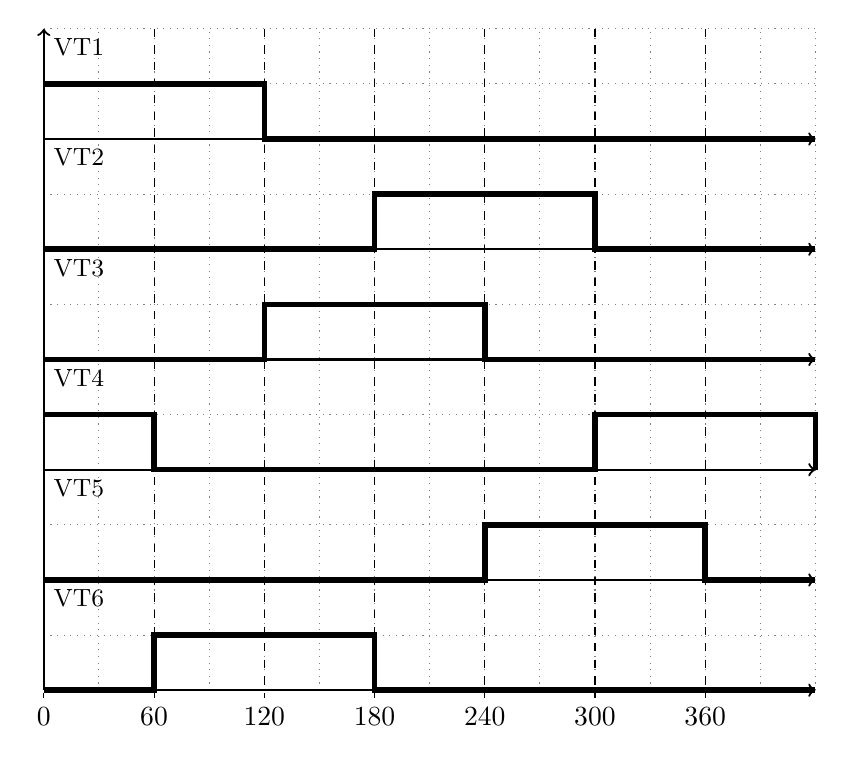
\begin{tikzpicture}
		\draw[gray, dotted, step = 0.7cm] (0, 0) grid (9.8, 8.4);
		\draw[dashed] (8.4, 8.4) -- (8.4, -0.1) node[anchor = north] {360};
		\draw[dashed] (7, 8.4) -- (7, -0.1) node[anchor = north] {300};
		\draw[dashed] (5.6, 8.4) -- (5.6, -0.1) node[anchor = north] {240};
		\draw[dashed] (4.2, 8.4) -- (4.2, -0.1) node[anchor = north] {180};
		\draw[dashed] (2.8, 8.4) -- (2.8, -0.1) node[anchor = north] {120};
		\draw[dashed] (1.4, 8.4) -- (1.4, -0.1) node[anchor = north] {60};
		\draw[dashed] (0, 8.4) -- (0, -0.1) node[anchor = north] {0};
		% Axis
		\draw[thick, ->] (0, 0) -- (0, 8.4);
		\draw[thick, ->] (0, 0) -- (9.8, 0);
		\draw[thick, ->] (0, 1.4) -- (9.8, 1.4);
		\draw[thick, ->] (0, 2*1.4) -- (9.8, 2*1.4);
		\draw[thick, ->] (0, 3*1.4) -- (9.8, 3*1.4);
		\draw[thick, ->] (0, 4*1.4) -- (9.8, 4*1.4);
		\draw[thick, ->] (0, 5*1.4) -- (9.8, 5*1.4);
		% Graph 1
		\draw[line width = 2] (0, 0) -- (1.4, 0) -- (1.4, 0.7) -- (4.2, 0.7) -- (4.2, 0) -- (9.8, 0);
		\draw[line width = 2] (0, 1.4) -- (5.6, 1.4) -- (5.6, 2.1) -- (8.4, 2.1) -- (8.4, 1.4) -- (9.8, 1.4);
		\draw[line width = 2] (0, 3.5) -- (1.4, 3.5) -- (1.4, 2.8) -- (7, 2.8) -- (7, 3.5) -- (9.8, 3.5) -- (9.8, 2.8);
		\draw[line width = 2] (0, 4.2) -- (2.8, 4.2) -- (2.8, 4.9) -- (5.6, 4.9) -- (5.6, 4.2) -- (9.8, 4.2);
		\draw[line width = 2] (0, 5.6) -- (4.2, 5.6) -- (4.2, 6.3) -- (7, 6.3) -- (7, 5.6) -- (9.8, 5.6);
		\draw[line width = 2] (0, 7.7) -- (2.8, 7.7) -- (2.8, 7) -- (9.8, 7);
		% Labels
		\draw (0, 1.4) node[anchor = north west] {\small VT6};
		\draw (0, 2.8) node[anchor = north west] {\small VT5};
		\draw (0, 4.2) node[anchor = north west] {\small VT4};
		\draw (0, 5.6) node[anchor = north west] {\small VT3};
		\draw (0, 7) node[anchor = north west] {\small VT2};
		\draw (0, 8.4) node[anchor = north west] {\small VT1};    
	\end{tikzpicture}
	\vspace{0.5cm}
	\caption{Эпюры переключения транзисторов}
\end{figure} \par

\newpage


\end{document}